\section{Inferential Methods}

\subsection{Estimation}
\begin{objectives}
    \item Understand the variability of a sample data
    \item Understand Confidence Level
    \item Know how to estimate Population mean with confidence level
\end{objectives}

\subsubsection{Variability of a Sample}
The values in a sample data vary slightly, the population's value even change more.The \Index{sampling variability} of a statistic refers to how much the statistic varies from sample to sample and is usually measured by its standard error
\begin{description}
    \item[Standard Error]a measure of the accuracy of predictions
    \begin{equation}
\sigma =\sqrt[2]{\frac{\Sigma (x\minus \bar x)^{2}}{n}}.
\end{equation}
    \item[Standard Deviation for sample]
    \begin{equation}
    \sigma_{\bar x} = \frac{\sigma}{\sqrt{n}} 
\end{equation}
    \item[Z score] is one type of measure of relative standing. It shows that how many standard deviation away from the mean a value is.
    \begin{equation}
      z=\frac{\bar x-\mu}{\sigma}
    \end{equation}
    \begin{examplebox}{Z score}
      If the population has a mean of 1.0 and a standard deviation of 0.2. Then a data with Z as 1 would has the value of 1.2 which is 1 standard deviation away from the population mean.
    \end{examplebox}
    \item[\Index{Central Limit Theorem}]:  When n is large and the sample size is less than 10 percent of the population size, the statistic
has a sampling distribution that is approximately
normal with mean.
    \item[\Index{Normal Distribution}]: Normal distributions are continuous probability distributions that are bellshaped and symmetric. There are many normal distributions, the \Index{Standard Normal Distribution} has Mean of 0, Standard Deviation of 1.
    \begin{figure}[H]
      \centering
    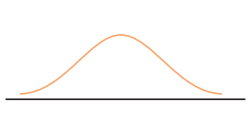
\includegraphics[width=75mm]{normald.png}
    \caption{A Normal distribution}
    \label{Figure}
\end{figure}
    \item[Empirical Rule]:The shape of a normal sampling distribution is defined by \Index{the empirical rule}. The is the statistical rule stating that for a normal distribution, then
Approximately 68\% of the observations are within 1 standard deviation of the
mean.
Approximately 95\% of the observations are within 2 standard deviations of the
mean.
Approximately 99.7\% of the observations are within 3 standard deviations of
the mean.
\begin{figure}[H]
      \centering
    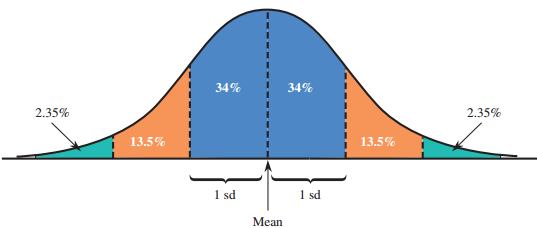
\includegraphics[width=95mm]{er.png}
    \caption{Empirical Rule}
    \label{Figure}
\end{figure}
\end{description}
\begin{Question}
    What if we want to know other percentage of observations correlated to other standard deviation? 
    \solution Use the Calculator.
\end{Question}

\subsubsection{Estimation of Confidence Interval}


\begin{description}
    \item \Index{Confidence Interval}: a confidence interval (CI) is a type of interval estimate of a population parameter.
    \item \Index{Confidence Level}: Confidence level is how frequently the observed interval contains the true parameter if the experiment is repeated, basically how "confident" we are about this estimation.
\\
\begin{examplebox}{Confidence Interval}
    If there is a sample data, we estimate its Confidence Interval for population's mean is 99 to 101 with a Confidence Level of 99\%, then it means we are 99\% sure the true mean of the population is within this range.
\end{examplebox}
\end{description}
 
\paragraph{How to calculate Confidence Interval} To calculate a confidence interval of a certain sample, we use an equation. However the equation varies when the standard deviation \(\sigma\) of the population is know or unknown.
\begin{description}
    \item \textbf{\(\sigma\) is known}:
    We use Z score to estimate.
    \begin{equation}
    \mu=\bar x \pm Z_{c} (\frac{\sigma}{\sqrt{n}} )
    \end{equation}
    \item \textbf{\(\sigma\) is unknown or n<30}:
    We use \Index{t distribution} which is more biased and vary more than normal distribution because the sample size is too small.
    \begin{equation}
    \mu=\bar x \pm t_{c} (\frac{\sigma}{\sqrt{n}} )
    \end{equation}
\end{description}

 \Index{Marginal Error}:It is the deviation the mean can have within a range.
 \begin{equation}
   M.E.= Z_{c} (\frac{\sigma}{\sqrt{n}} )
\end{equation}
\paragraph{How to get \(z_c\) or \(t_c\)}In order to get \(z_c\) and \(t_c\), we use the given confidence level. 
\begin{figure}[H]
      \centering
    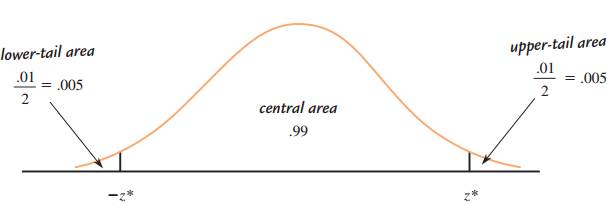
\includegraphics[width=95mm]{meanestimate.png}
    \caption{Confidence Interval}
    \label{Figure}
\end{figure}
\begin{examplebox}{Get \(z_c\)}
    If the confidence level is 90\%, then it means the confidence level should cover 90\% of the area in a sample's distribution curve, then we use this information to type in calculator to get it.
\end{examplebox}

\begin{Question}
    How about t distribution
    \solution Use the t-dis button on the calculator and do the same thing
\end{Question}

\subsection{Hypothesis Test}
\begin{objectives}
    \item Know Null hypothesis
    \item Distinguish \(H_a\) and \(H_0\) hypothesis
    \item Know how to test hypothesis with \(z_c\) and z
    \item Know p-value as significance level
\end{objectives}
\vbox{}
We have use a sample and its values to infer its population's mean.

\subsubsection{Hypothesis}
\Index{Hypothesis}: A hypothesis is a claim or statement about the value of a single population characteristic or the values of several population characteristics. 
\begin{itemize}
    \item \Index{Null Hypothesis}: The null hypothesis, denoted by \(H_0\), is a claim about a population characteristic that is initially assumed to be true.
    \item \Index{Alternative Hypothesis}: denoted by \(H_a\), is the competing claim.
\end{itemize}
\begin{examplebox}{Hypothesis}
    \(H_a\): \(\mu <3\) \\
    \(H_0\): \(\mu =3\)
\end{examplebox}

\subsubsection{Errors in Hypothesis Testing}
In this section, we discuss
the kinds of errors that can occur and consider how the choice of a test procedure
influences the chances of these errors.
\begin{description}
    \item[\Index{Type I Error}]: the error of rejecting \(H_0\) when \(H_0\) is true.The \textbf{\Index{probability of a type I error occurs}} is denoted by \(\alpha\)
    \begin{center}
        \(\alpha\)=P( reject \(H_{0}\) | \(H_{0}\) is true)
    \end{center}
    \item[\Index{Type II Error}]:the error of failing to reject \(H_0\) when \(H_0\) is false.The \textbf{\Index{probability of a Type II error}} is denoted by \(\beta\).
    \begin{center}
        \(\beta\)=P( fail to reject \(H_{0}\) | \(H_{0}\) is false)
    \end{center}
\end{description}
\begin{examplebox}{Error}
    A researcher wants to compare the speed  of two cars. The null and alternative hypotheses are:
\begin{itemize}
    \item Null hypothesis (\(H_{0}\)): \(\mu_{1}=\mu_{2}\); The two cars are the same fast
\item Alternative hypothesis (\(H_{a}\)): \(\mu_{1}\neq \mu_{2}\); The two cars are not the same fast.
\end{itemize}
A type I error occurs if the researcher rejects the null hypothesis and concludes that the two cars are different but in fact they are not.  \\
A type II error occurs if the researcher fails to reject the null hypothesis when it should be rejected. That is, the researcher concludes that the cars are the same when, in fact, they are different. 
\end{examplebox}

\subsubsection{Testing Hypothesis}
Now that the basic concepts of hypothesis testing have been introduced, we are ready
to turn our attention to the development of procedures for using sample information
to decide between a null and an alternative hypothesis. There are two possible conclusions: We either reject \(H_0\) or we fail to reject \(H_0\).
\\
\begin{description}
    \item[\Index{P-Value or Observed Significance Level}]: A measure of inconsistency between the hypothesized value for a population characteristic and the observed sample. It is the probability, assuming that \(H_0\) is true,
of obtaining a test statistic value at least as inconsistent with \(H_0\) as what was
observed.
    \item[\Index{Significance Level}]: The significance level is the highest value of a probability value for which the null hypothesis is rejected.
    \item[\Index{Test Statistic}]: A test statistic is computed using sample data and is the value used to reach a
conclusion to reject or fail to reject \(H_0\).
\end{description}

\paragraph{How to test}: Depending on the \(H_a\), we have \Index{One tail test} and \Index{Two tail test}

\begin{figure}[H]
    \centering
    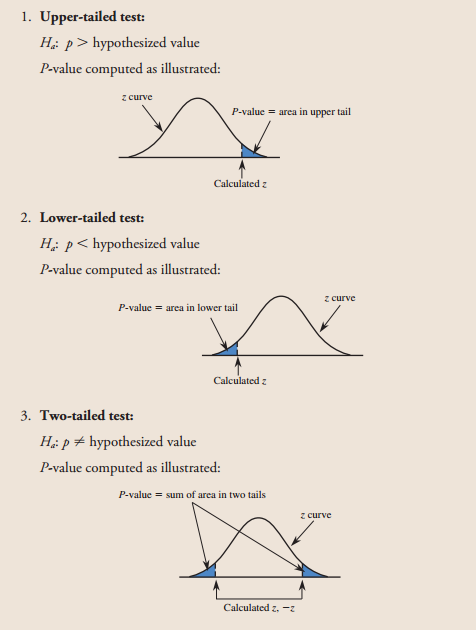
\includegraphics[width=125mm]{testhp.png}
    \caption{One-tail Test and Two-tail Test}
    \label{Figure 2}
\end{figure}

\textbf{Steps on Testing}
\begin{enumerate}
    \item Describe the population characteristic about which hypotheses are to be tested
    \item State the null hypothesis \(H_0\).State the alternative hypothesis \(H_a\).
    \item Select the significance level a for the test.
    \item Display the test statistic to be used, with substitution of the hypothesized
value identified in Step 2 but without any computation at this point.
    \item Check to make sure that any assumptions required for the test are reasonable.
    \item Compute all quantities appearing in the test statistic and then the value of
the test statistic itself.
    \item Determine the P-value associated with the observed value of the test statistic.
    \item State the conclusion 
    \begin{itemize}
    \item \textbf{If p-value<\(\alpha\), then we reject \(H_0\)}
    \item \textbf{If p-value>\(\alpha\), then we fail to reject \(H_0\)}
\end{itemize}
\end{enumerate}

\begin{Question}
    Are \(\alpha\) and Confidence Level connected?
    \solution The confidence interval at confidence level \(1-\alpha\%\) for a population statistic contains \(1-\alpha\%\) of data. So for example, the significance level is 5\% if the confidence level is 95\%
\end{Question}
\subsubsection{Power}
\Index{Power of a Test}: The power of a test is the probability of rejecting the null hypothesis
\begin{equation}
    Power=1-\beta
\end{equation}
\begin{center}
    \(1-\beta\)=P( reject \(H_{0}\) | \(H_{0}\) is false)
\end{center}
\begin{figure}[H]
    \centering
    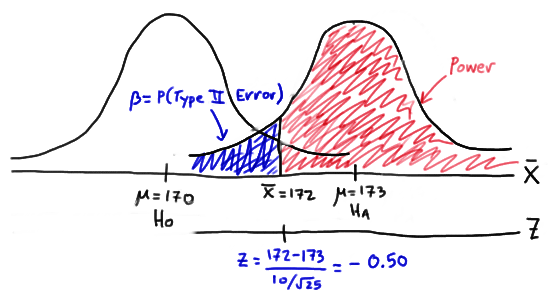
\includegraphics[width=110mm]{power.png}
    \caption{Power}
    \label{Figure}
\end{figure}
\begin{Question}
    How do get p-value?
    \solution we use the corresponding Z to type into calculator to get the area of the uncovered area.
\end{Question}

\subsection{Sample Size}
\begin{objectives}
    \item Understand the effect of sample size on sample
    \item Know how to calculate the smallest sample size to get a certain Margin Error
\end{objectives}
\vbox{}
The sample size n is very important to a sample data's distribution, the bigger n becomes, the more normal the distribution become and the closer the data is to the true population mean.\\
\vbox{}
So,the bigger the sample size, the smaller the Margin error becomes.\\
\vbox{}
From the previous chapter, we know the equation of Marginal Error is
\begin{equation}
   M.E.= Z_{c} (\frac{\sigma}{\sqrt{n}} )
\end{equation}
If we change the equation and solve for n, we get the following equation for n
\begin{equation}
    n=\frac{z^{2}\times \sigma^{2}}{(M.E.)^{2}}
\end{equation}
\begin{examplebox}{Minimum Sample Size}
    Q: We want to estimate the average age of the workers, to \(\pm 1 year\), with a confidence level of 95\%. The standard deviation of the poupulation is 0.1.How big should the sample be? \\
According to the question, we can know the given value, M.E.=\(1 year\) and C.L.=\(0.95\). \\
Use the C.L. to get the Z value with calculator.\\
Plug these number in the equation \(n=\frac{z^{2}\times \sigma^{2}}{(M.E.)^{2}}\)\\
Then roung n to the nearest integer.
 
\end{examplebox}